\documentclass{article}

\usepackage[preprint]{neurips_2018}

\usepackage[utf8]{inputenc}
\usepackage[T1]{fontenc}
\usepackage{amsfonts}
\usepackage{booktabs}
\usepackage{bm}
\usepackage{caption}
\usepackage{float}
\usepackage{graphicx}
\usepackage{hyperref}
\usepackage{microtype}
\usepackage{natbib}
\usepackage{nicefrac}
\usepackage{url}

\title{Reproducing \textit{Colorful Image Colourization}}

\author{%
  Timo Nicolai \\ \texttt{tnicolai@kth.se}
  \And
  Álvaro Orgaz Expósito \\ \texttt{alvarooe@kth.se}
  \And
  Carolina Bianchi \\ \texttt{cbianchi@kth.se}
}

\begin{document}

\maketitle

\begin{abstract}
In this project we reproduce part of the work presented by Zhang et al. in
\textit{Colorful Image Colorization}~\cite{Zhang2016}. We implement their
network architecture from scratch in \textit{PyTorch}~\cite{PyTorch} and train
it on a subset of ImageNet~\cite{ImageNet}. We find that our network is able to
produce realistic colourizations on par with the reference implementation
provided by Zhang et al. in many cases. We further describe several experiments
that support this conclusion, providing quantitative metrics for the closeness
between colourizations produced by our network and corresponding ground truth
images. We also show how, in some cases, our network is able to fool human
testers in a perceptual realism study. Finally we show that our network can
improve greyscale image classification accuracy when employed as a
preprocessing step.
\end{abstract}

\section{Introduction}

Greyscale image colourization has been a longstanding topic of interest in the
computer vision and machine learning communities. The principle problem is to
\textit{plausibly} colourize greyscale input images, implying that the results
do not necessarily have to match the ``correct'' colours for any given image.
Instead they only have to be believable, i.e. able to fool humans observers
into mistaking them for real colour images.

Besides its appeal in areas such as the colourization of historical images,
colourization networks can also serve as a preprocessing step for image
classification and segmentation networks or be used in transfer learnings tasks.
A possible commercial application is the improvement of surveillance systems
without hardware upgrades.

The problem of colourization is clearly under-constrained and ill-posed: many
objects could be plausibly coloured in multiple different ways. This inherent
multimodality suggests the use of a network that predicts a distribution of
possible colours for each pixel which can then be converted into a suitable
point estimate (e.g. the distributions mean or mode).

The multimodality of the problem also makes assessing a method's performance
difficult: metrics that simply measure some form of distance between ground
truth and prediction provide limited insight into the plausibility of the
latter. Under such metrics, methods producing conservative (i.e. desaturated)
results often outperform methods producing more vibrant images whose colour
scheme differ from the ground truth but remain similarly plausible. The
plausibility of colourized images can thus be most reliably assessed by human
testers.

In section 2 we first provide a short overview of related previous and current
approaches to the colourization problem. Section 3 describes the datasets which
we utilized to train our network. Section 4 provides a summary of the
method developed by Zhang et al.~\cite{Zhang2016} on which our work is based.
In section 5 we describe how we trained our network and present some exemplary
results as well as the outcome of a perceptual realism study with human
testers. Here we also evaluate how preprocessing greyscale images using our
network can lead to improved image classification results.

\section{Related work}

Image colourization has been well studied in the literature. Here we provide an
overview of major previous and current approaches with a focus on (deep)
learning based methods.

Very early work in this field was performed by Welsh et al.~\cite{Welsh2002}
whose approach transferred colours from an existing reference image through
matching of luminance information and texture.

Shortly thereafter Levin et al.~\cite{Levin2004} formulated colourization as an
optimization problem and designed a loss function which penalizes colour
differences between neighboring pixels of similar intensity. However, their
approach required user annotation to produce acceptable results.

Early learning based approaches include work by Deshpande et
al.~\cite{Deshpande2015} who implemented colourization by training a linear
system and work by Cheng et al.~\cite{Cheng2015}  who utilized a multi-layer
fully connected neural network.

Zhang et al.~\cite{Zhang2016} leveraged large-scale data and a deep (almost)
end-to-end trainable convolutional neural network. Similar methods were
developed concurrently by Larsson et al.~\cite{Larsson2016} and Iizuka et
al.~\cite{Iizuka2016}. These mainly differ in the utilized network
architectures and loss functions, i.e. $L_2$ reconstruction loss (Iizuka et
al.) and classification loss (Zhang et al, Larsson et al.).

More recent approaches include work by Nazeri et al.~\cite{Nazeri2018} which
leverages Deep Convolutional Generative Adversarial Networks in order to learn
both a mapping from lightness input to colour output and a loss function via a
discriminator network. This is in turn based on prior work by Isola et
al.~\cite{Isola2016} and mainly improves on the proposed training approach and
generalizes it to higher resolution images.

An interesting variant of the colourization problem is exemplar-based
colourization in which the colourization is aided by a user provided reference
image. A deep learning approach was first applied to this problem by He et
al.~\cite{He2018}. The authors also describe an image retrieval
algorithm that can automatically determine suitable reference images. The key
advantage of this approach is that by selecting different references, more than
one plausible colourization can be produced per input image.

\section{Data}

We work with images in the Lab colour space, in which each pixel is
encoded by three values: its lightness (black to white), its a* value (green
to red) and its b* value (blue to yellow). This colour space was originally
designed such that the distances within it roughly correspond to perceptual
``distances''~\cite{LAB}, making it especially well suited for tasks such as
this where the ultimate aim is to fool the human eye.

The image colourization task has the appealing property that any colour image is
a potential self labeled training sample. After converting it into the Lab
colour space, its lightness channel can serve as a network input and its a and
b channels as supervisory signal.

To train the our network we decided to use a subset of the
ImageNet~\cite{ImageNet} training set. We created this subset by first choosing
$33$ semantically closely related\footnote{We defined closeness via
WordNet~\cite{WordNet} path similarity, see
\href{http://www.nltk.org/howto/wordnet.html}{http://www.nltk.org/howto/wordnet.html}.}
synsets from the $1000$ synsets making up the complete training set. These
include $42,556$ images of mostly fruits and vegetables.

Our motivation for this was twofold: Firstly, a training set made up of few,
visually related objects is likely to speed up generalization to test images
depicting similar objects. Secondly, most images in the synsets we chose depict
objects with distinct and vibrant colours and easily identifiable textures.
These make for excellent examples when demonstrating our networks performance
in section 5.

We do not employ a validation set. Even though our training set is relatively
small, overfitting is unlikely because of the short training time and
appropriate regularization.

In accordance with Zhang et al. we resize all images in the training set to
$256 \times 256$. During training, these are randomly cropped to $176 \times 176$
and mirrored horizontally with probability $0.5$.

\section{Methods}

\subsection{Loss function}

Starting from an image of size $H \times W$ in the Lab colour space, we use its
luminance channel $X_L \in \mathbb{R}^{H \times W \times 1}$ as input to our
network, which we train to estimate the remaining channels ($X_a, X_b$) in
order to generate a fully coloured version of the image $X=(X_L, X_a, X_b)$.

Given the input lightness channel the objective is to learn a mapping
$\hat{X}_{ab} = F(X_L)$ to the two associated colour channels $X_{ab} \in
\mathbb{R}^{H \times W \times 2}$. A natural objective function would be the
Euclidean distance $L_2$ between the predicted and ground truth colours of each
pixel. However, due to the multimodal nature of the colourization problem, we
can achieve more vibrant results using a classification loss. The classes in
question result from the quantization of the original \textit{ab} output space
into bins of size $10 \times 10$. $Q = 313$ of these bins are
\textit{in-gamut}, i.e.  representable in the sRGB colour space.

The network predicts the per pixel colour probability distribution $\hat{Z} \in
[0,1]^{H\times W \times Q}$. More specifically, for every pixel of the input
image (after several downsampling steps) the network outputs $Q$ values which
roughly correspond to the log probabilities of the \textit{ab} value associated
with that pixel falling into the respective bins.  This distribution can be
converted back to the original \textit{ab} space by taking its
\textit{annealed-mean} as described below.

In order to train the networks parameters we additionally need to convert the
ground truth images \textit{ab} channels into a ground truth distribution $Z$.
It would be reasonable to encode the ground truth value of each pixel as a
1-hot vector $Z_{h,w}$ of length $Q = 313$ by searching for the nearest quantized
\textit{ab} bin. Instead we employ the soft-encoding scheme proposed by Zhang
et al. which encodes every pixel by its five nearest neighbours in the binned
\textit{ab} space, weighted proportionally to their distance from the ground
truth values using a Gaussian kernel with $\sigma = 5$. This allows the network
to learn relationships between elements in the output space more easily.

Finally, the model parameters are optimized by minimizing the multinomial
cross entropy loss defined in equation \ref{eq:loss}.

\begin{equation}
L(Z, \hat{Z}) = -\sum_{w,h} v(Z_{w,h}) \sum_q Z_{w,h,q} \cdot log(\hat{Z}_{w,h,q})
\label{eq:loss}
\end{equation}

Here, $v(Z_{h,w})$ is a weighting term that rebalances each pixel's
contribution based on the rarity of its closest \textit{ab} bin. More
specifically, Zhang et al. provide a \textit{ab} bin prior distribution
$\tilde{\bm{p}}$ calculated from all images in ImageNet. The weights are then
chosen as a mixture of this prior and a uniform distribution over all
\textit{ab} bins, i.e.:

\begin{equation}
v(Z_{w,h}) \propto \left((1 - \lambda) \tilde{\bm{p}} + \frac{\lambda}{Q} \right)^{-1}
\label{eq:rebal}
\end{equation}

In practice this reweighting is implemented by a custom PyTorch layer which,
on every backward pass, multiplies the per pixel gradients by the weighting
terms which are recalculated on the GPU for each input image.

This class rebalancing is crucial in order to achieve plausible colourizations
since the distribution of colours in natural images is strongly biased towards
low \textit{ab} values (mostly due to background objects such as clouds,
pavement, dirt, walls etc.). Without rebalancing the loss function is dominated
by desaturated \textit{ab} values and network outputs are significantly less
vibrant.


\subsection{From colour probabilities to point estimates}

In order to convert the distribution $\hat{Z}$ into point estimates in
the original \textit{ab} space $\hat{X}_{ab}$ we implement the annealed-mean
operation in equation \ref{eq:ann_mean}.

\begin{equation}
H(Z_{h,w}) = E[f(Z_{h,w})] \qquad f(z) = \frac{exp(log(z)/0.38)}{\sum_q exp(log(z)/0.38)}
\label{eq:ann_mean}
\end{equation}

Through this operation it possible to make a trade off between the mean and
mode of the predicted output distribution. The former often leads to spatially
consistent but desaturated images and the latter to vibrant images containing
unwanted image artefacts (patches of high saturation).  Setting $T = 0.38$ as
suggested by Zhang et al. offers a nice compromise between the two.

Figure~\ref{fig:annealed_mean} demonstrates how adjusting the
temperature parameter results in a trade-off between mean and mode of the
colour bin distribution predicted by our network.

\begin{figure}
    \centering
    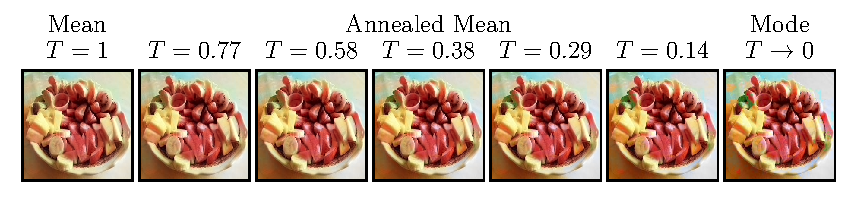
\includegraphics[width=\textwidth]{resources/annealed_mean.pdf}
    \caption{Effect of temperature parameter on network output. Note how higher
             values of $T$ results in a less vibrant but more spatially
             consistent image.}
    \label{fig:annealed_mean}
\end{figure}


\subsection{Network architecture}

Table~\ref{tbl:arch} lists our network architecture.\footnote{$C$ = number of
filters, $S$ = stride, $D$ = dilation, $BN$ = batch normalization, $K$ =
filter diameter} It is adapted from Figure 2 in~\cite{Zhang2016}, activation
layers are not depicted. Downsampling is achieved with strided convolutions
(i.e. without pooling layers). Also note the dilated (otherwise referred to as
atrous) convolution layers which increase the receptive field of the trained
convolution kernels without an explosion in the number of parameters.

\begin{table}
  \centering
  \caption{Network architecture}
  \label{tbl:arch}
\begin{minipage}[t]{.4\textwidth}
  \vspace{10pt}
  \begin{tabular}{llllll}
    \toprule
    Layer     & C   & S & D & BN & K\\
    \midrule
    \midrule
    conv1\_1  & 64  & 1  & 1 & - & 3 \\
    conv1\_2  & 64  & 2  & 1 & $\checkmark$ & 3 \\
    \midrule
    conv2\_1  & 128 & 1  & 1 & - & 3 \\
    conv2\_2  & 128 & 2  & 1 & $\checkmark$ & 3 \\
    \midrule
    conv3\_1  & 256 & 1  & 1 & -            & 3 \\
    conv3\_2  & 256 & 1  & 1 & -            & 3 \\
    conv3\_3  & 256 & 2  & 1 & $\checkmark$ & 3 \\
    \midrule
    conv4\_1  & 512 & 1  & 1 & -            & 3 \\
    conv4\_2  & 512 & 1  & 1 & -            & 3 \\
    conv4\_3  & 512 & 1  & 1 & $\checkmark$ & 3 \\
    \midrule
    $\vdots$ & $\vdots$ & $\vdots$ & $\vdots$ & $\vdots$ & $\vdots$
  \end{tabular}
\end{minipage}%
\begin{minipage}[t]{.4\textwidth}
  \vspace{0pt}
  \begin{tabular}{lllllllll}
    $\vdots$ & $\vdots$ & $\vdots$ & $\vdots$ & $\vdots$ & $\vdots$ \\
    conv5\_1  & 512 & 1  & 2 & -            & 3 \\
    conv5\_2  & 512 & 1  & 2 & -            & 3 \\
    conv5\_3  & 512 & 1  & 2 & $\checkmark$ & 3 \\
    \midrule
    conv6\_1  & 512 & 1  & 2 & -            & 3 \\
    conv6\_2  & 512 & 1  & 2 & -            & 3 \\
    conv6\_3  & 512 & 1  & 2 & $\checkmark$ & 3 \\
    \midrule
    conv7\_1  & 512 & 1  & 1 & -            & 3 \\
    conv7\_2  & 512 & 1  & 1 & -            & 3 \\
    conv7\_3  & 512 & 1  & 1 & $\checkmark$ & 3 \\
    \midrule
    conv8\_1  & 256 & .5 & 1 & -            & 4 \\
    conv8\_2  & 256 & 1  & 1 & -            & 3 \\
    conv8\_3  & 256 & 1  & 1 & -            & 3 \\
    \midrule
    conv9\_1  & 313 & 1  & 1 & -             & 1 \\
    \bottomrule
  \end{tabular}
\end{minipage}
\end{table}

\section{Experiments}

\subsection{Training}

Because extensive search for good optimization hyperparameters would have been
prohibitively expensive given the available GPU resources, we simply applied
the same optimization regimen used by Zhang et al. to train their
\href{https://github.com/richzhang/colorization}{publicly available
models}.\footnote{ADAM~\cite{Adam} optimizer with $\beta_1 = .9$, $\beta_2 =
.99$, weight decay = $10^{-3}$, $\eta = 3.16e \times 10^{-5}$, batch size =
$40$.} We also utilized class rebalancing with $\lambda = 0.5$.

We trained our network for $150,000$ iterations which took approximately $20$
hours on an \textit{NVIDIA Tesla V100}.

\subsection{Examples}

The trained network produces results which are in many cases obviously fake.
Nevertheless, the network seems to consistently apply realistic and vibrant
colours to certain prominent objects that are abundant in the training set such
as bananas or blooming artichokes. Figure~\ref{fig:good_vs_bad} shows some test
set images for which our network performs especially well.

We believe that the achieved vibrancy is a result of class rebalancing and that
the overall lackluster network performance is caused by the challenging nature
of the chosen dataset which contains many colourful and visually very different
objects (unlike images of natural scenes on which the network trained by Zhang
et al. performs especially well and which are mostly composed of large areas
homogeneous in texture and colour, such as forest, sea and air).

\begin{figure}
    \centering
    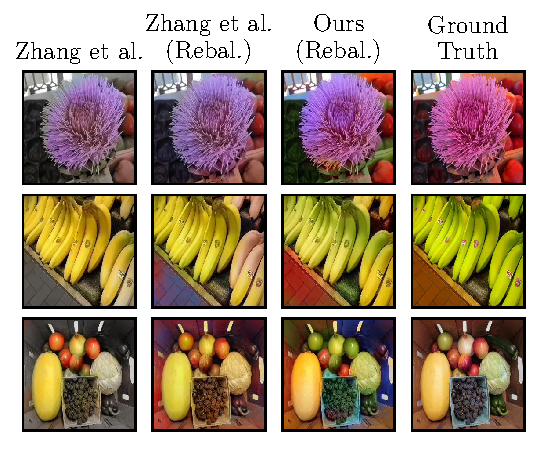
\includegraphics{resources/good_vs_bad.pdf}
    \caption{Particularly good examples where our network produces more vibrant
             and realistic colours than the pretrained models provided by Zhang
             et al. trained on the full ImageNet training set.}
    \label{fig:good_vs_bad}
\end{figure}

\subsection{Perceptual realism study}

To test whether the colour images produced by our network are realistic enough
to fool the human eye, we colourized fifty images from the ImageNet validation
set (from the same synsets making up the training set) and presented them to
ten volunteers alongside the corresponding ground truth images, displaying each
of these in turn for exactly one second. The volunteers were then given
unlimited time to identify the real ground truth image.

Figure~\ref{fig:amt_results} displays the images which fooled the greatest
number of participants and a selection of those which were never mistaken for
the ground truth image. On average, participants were fooled $18.78\%$ of the
time indicating that while our network is able to produce realistic
colourization in some ``easy'' cases, results are mostly obviously artificial.

\begin{figure}
    \centering
    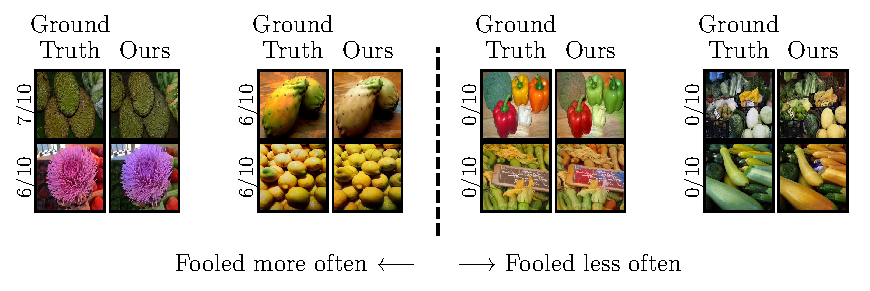
\includegraphics[width=\textwidth]{resources/amt_results.pdf}
    \caption{User study results, labels indicate how many volunteers were fooled
             by the corresponding image.}
    \label{fig:amt_results}
\end{figure}

\subsection{Colourization accuracy and semantic interpretability}

We made use of the \textit{area under curve} (AuC) metric introduced
in~\cite{Deshpande2015} to also obtain a quantitative measure of how close the
results produced by our network are to the ground truth.  Zhang et al. improve
on this metric by reweighting pixels by the inverse prior likelihood of the
colour bin into which they fall. This alleviates the comparatively better
results achieved when ``conservatively'' predicting images with low saturation
due to the prevalence of pixels with low saturation in natural images.

Additionally, in order to show that our results are not only visually
appealing but also suitable as inputs to classification networks trained on
colour images, we tested whether using our network as a preprocessing step
results in improved top-5 classification accuracy for a VGG-16~\cite{VGG}
network trained on the complete ImageNet training set.

We calculated the average AuC and top-5 classification accuracy for several
image set variants. To this end, we first randomly sampled a thousand images
belonging to twenty synsets from the ImageNet validation set. The twenty
synsets are a subset of the sysets from which we composed the training set.  We
then also converted these images to greyscale and reconstructed their colour
channels using both the trained network provided by Zhang et al. as well as our
trained network. To show that the semantic colourization learned by both
networks is superior to arbitrary (spatially consistent) colourization, we also
colourized the greyscale images by treating them as the L channel of an image
in the Lab colour space and appending the a and b channels from randomly chosen
ImageNet training set images.

\begin{table}
  \centering
  \caption{Quantitative coluorization results}
  \label{tbl:comp-results}
  \begin{tabular}{llll}
    \toprule
    Method        & Auc  & AuC (rebal.)  & VGG-16 Top-5 Acc. \\
    \midrule
    Ground truth  & 1    & 1             & 92.1 \\
    Grayscale     & 79.9 & 68.3          & 46.4 \\
    Random colour & 79.0 & 68.2          & 17.4 \\
    \midrule
    Zhang et al.  & 83.8 & 78.6          & 67.7 \\
    Ours          & 85.5 & 81.0          & 81.0 \\
    \bottomrule
  \end{tabular}
\end{table}

Table~\ref{tbl:comp-results} lists the average AuC obtained on the different
dataset variants. We find that, as expected, relative improvement in AuC for
colourized images compared to greyscale images is greater when applying
rebalancing.

Also listed are the top-5 classification accuracies we obtained. We find that
colourization significantly improves classification performance. This effect is
more pronounced for our network. We believe this is due to the smaller number
of distinct objects depicted in the reduced training set which allows our
network to mostly assigns very plausible colours to these primary objects
despite reduced training time. This is likely to have a larger positive
influence on classification than the plausible colourization of background
objects.

Figure~\ref{fig:vgg_classification_performance} displays classification
accuracy achieved for images colourized using our network, relative to
greyscale images, averaged over each of the twenty synsets present in the test
set. Colourization improves average accuracy in all twenty cases, especially
when accuracy on greyscale images is low to begin with.

\begin{figure}
\centering
\begin{minipage}[t]{.45\textwidth}
    \centering
    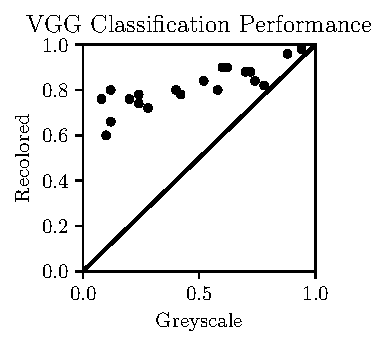
\includegraphics{resources/vgg_classification_performance.pdf}
    \captionof{figure}{Classification performance comparison for greyscale
                       images before and after colourization by our network,
                       averaged for twenty different synsets.}
    \label{fig:vgg_classification_performance}
\end{minipage}%
\qquad
\begin{minipage}[t]{.45\textwidth}
    \centering
    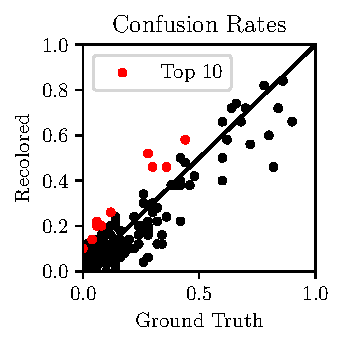
\includegraphics{resources/confusion_rates.pdf}
    \captionof{figure}{Distribution of off-diagonal confusion matrix entries.}
    \label{fig:confusion_rates}
\end{minipage}
\end{figure}

For some synsets colourization can amplify the occurence of certain confusions
cases during classification. To quantify this effect, we calculated the top-5
confusion matrices $C_{ground truth}$ and $C_{colourized}$ with entries
$C_{i,j}$ equal to the proportion of images with ground truth label $i$
for which $j$ is one of the five labels predicted as most likely.
Figure~\ref{fig:confusion_rates} displays the off-diagonal elements of
$C_{colourized}$ plotted over the corresponding elements of $C_{ground truth}$
with those for which the difference $C_{colourized} - C_{ground truth}$ is
largest highlighted.

\begin{figure}
    \centering
    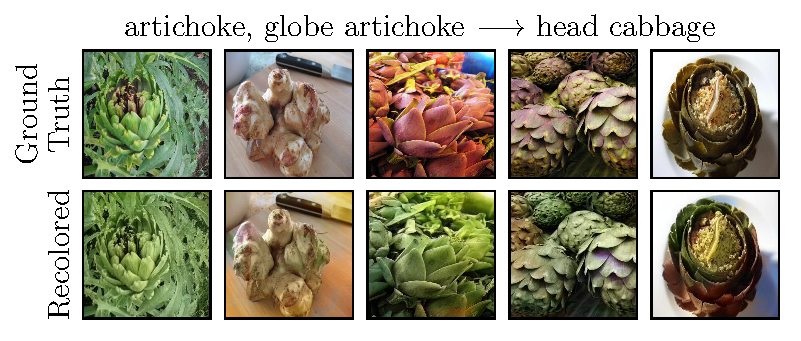
\includegraphics{resources/common_confusions.pdf}
    \caption{Confusion case most strongly amplified by colourization, note that
             both classes of objects are visually similar to begin with and a
             slight shift towards a ``greener'' palette is enough to cause the
             confusion to occur.}
    \label{fig:common_confusions}
\end{figure}

Clearly, colourization makes certain confusion cases more and others less
likely. Figure~\ref{fig:common_confusions} visualizes the confusion case for
which colourization results in the largest increase of the corresponding
confusion matrix entry. The images shown are those for which the confusion
occurs for those colourized from greyscale images but not for the corresponding
ground truth images.

\section{Conclusions}

Our work validates the image colourization approach employed by Zhang et al.
The network that we trained from scratch is able to determine suitable colours
for the most common fruits and vegetables, as proven by our user-study. This
suggests that our network has implicitly learnt to classify/segment input
images. It is thus feasible that the representations learnt by our network
could be useful in transfer learning tasks. Zhang et al. explore this
possibility in the original paper by successfully training linear classifiers
and segmentation networks on top of their trained colourization network.

However the network often fails in colourizing backgrounds objects: it tends to
produce coloured spots which are an obvious giveaway of
artificial colouring. To mitigate this effect, it would be interesting to
explore post-processing approaches based on enforcing spacial consistency
or to pre-process images via explicit segmentation into fore- and background
and use different networks to colourize both.

The measured improvement in classification accuracy for images which have
undergone the colourization process suggests that our network could be useful
as a preprocessing step in greyscale image classification tasks.

\small
\bibliographystyle{unsrt}
\bibliography{report}

\end{document}
